
\chapter{Neutron Skin Thickness Measurement} \label{intro}
\commento{
\begin{itemize}
\item explain neutron skin thickness.
\item connection to neutron stars radious, and neutron stars description.
\item Equation of state (EoS) for high density nuclear matter.
\item Parity-violating scattering experiment for extracting neutron skin thickness.
\item mention the weak form factor.
\item Transverse asymmetry as background for Parity-violating experiment. 
\item Mention the other experiment, like PREX, that measure zero $A_{n}$ for Lead.
\end{itemize}}

\section{The Mainz Radius Experiment}

The Mainz Radius Experiment (MREX), at the Mainz nuclear physics institute, is an experimental campaign with the aim of investigating the nature of atomic nuclei, by measuring the neutron skin thickness of $^{208}Pb$. The characteristics of atomic nuclei are mainly determined by the strong interaction, whose existence was firstly speculated by Yukawa in 1935. The strong interaction is responsible of a broad range of phenomena: from the nature of the nuclei, the compositions of baryons and meson to the exotic structure of Neutron stars. Hence, nuclear physics offers many answers to fundamental questions that are important also in other fields of physics. The neutron stars, which are among the most researched astrophysical objects, are particularly well suited to study theories of dense nuclear matter. It can be surprising to think that, despite having differences of so many orders of magnitude, neutron rich nuclei and neutron stars share the same fundamental physics description, given by the the Equation Of State (EOS) of nuclear matter \cite{Thiel_2019}. The Equation Of State represents the fundamental relation between the state variables such as temperature, energy, pressure and the neutron-proton asymmetry. Specifically, the goal of the MREX experiment is to determine an important parameter of the EOS, the slope of the symmetry energy at saturation density $L$, which controls the change in energy due to presence of an asymmetry between neutron and proton densities. This parameters plays an important role for the determination of the radius of the neutron stars and it is also responsible for a peculiar characteristic shown by heavy nuclei: the neutron skin thickness. The neutron skin thickness $\delta r_{np}$ is a phenomena that affect heavy nuclei, which consists in the accumulation of the excess of neutrons near the surface, producing a neutral layer of neutrons. It is defined as: 

\begin{equation} \label{eq:NeutronSkin}
\delta r_{np} = \sqrt{\vphantom{r^{2}_{p}}<r^{2}_{n}>} - \sqrt{<r^{2}_{p}>} ,
\end{equation}

Where $<r^{2}>_{n}$ and $<r^{2}>_{p}$ are the rms radii of proton and neutron distributions. The neutron skin thickness is sensitive to $L$, so an accurate determination of $\delta r_{np}$ provides significant constrains on the value of $L$, which can be used as an input to many theoretical models of the structure of the neutrons stars.
There are numerous challenges in determining $\delta r_{np}$. $r_{p}$ is measured with high accuracy with the electrons elastic scattering experiments, whereas the determination of $r_{n}$ has traditionally relied on hadronic experiments, such as proton-nucleus scattering, $\pi^{0}$ photo-production, $\alpha$ and $\pi$ nucleus scattering. These processes suffer from large and often uncontrolled theoretical uncertainties that compromise the extraction of the neutron density. The most promising method, that is the least model dependent, is parity-violating electron scattering, where longitudinal polarized electrons are elastically scattered off an unpolarized target. This method consists in the measurement of the cross-section asymmetry between right and left handed electrons:

\begin{equation}
A_{pv} = \dfrac{\sigma_{R} - \sigma_{L}}{\sigma_{R} + \sigma_{L}}
\end{equation}

This process is dominated by the exchange of a virtual photon, which is sensitive to the charge form factor, and of a $Z_{0}$ boson, that is sensitive to the weak form factor. Since the weak charge of the neutron is $Q_{w} = 0.99$ and the weak charge of the proton is $0.04$, the weak form factor contains the information on the neutron density, necessary to measure $\delta r_{np}$. In this context, the MREX experiment is an experimental campaign with the aim of measuring the neutron skin thickness via the parity violating scattering with the new MESA electron accelerator, at the nuclear physics institute of Mainz.

\section{Nuclear Equation of State (EOS) and Neutron Skin Thickness}

\commento{In this section we have to explain what is the neutron skin thickness and why this parameter is related to the Equation of State for nuclear matter (in particular, the slope of the Symmetry energy in the semiempirical mass formula). Then, explain the parallelism between Neutron stars and Nuclear matter (the share the same EOS), and underline the relation between radius of the neutron stars and EOS.}

During the 30s of the last century, a considerable part of the scientific community was focused in the study of the structure of atomic nuclei. The discovery that every atoms has a positive charged nucleus dates back to 1908, with the famous Rutherford experiment, where alpha particles scatter on a thin gold foil. In the following years, especially after the birth of quantum mechanics in the second half of the 1920s, important progress was made in the knowledge of atomic nuclei and their properties. In 1935, a significant contribution was given by Carl Friedrich von Weizsäcker and Hans Bethe, who proposed the semi-empirical mass formula, to approximate the mass of an atomic nucleus \cite{Bethe:1936zz}. Although some refinements have been made over the years, the general structure of the formula is the same today. 
The model proposed by Weizsäcker is the application of the liquid-drop model for nuclear matter, where the nucleus is described as a drop of protons and neutrons, assumed to be incompressible and held together by a nuclear potential. The semi-empirical mass formula states that the mass of a nucleus with Z protons and N neutrons is given by: 

\begin{equation}
m = Zm_{p} + Nm_{n} - \frac{E_{B}(N,Z)}{c^{2}}
\end{equation}

where $E_{B}$ is the binding energy, containing 5 parameters:

\begin{equation}
E_{B} = a_{V}A -  a_{s}A^{\frac{2}{3}} - a_{c}\dfrac{Z^{2}}{A^{\frac{1}{3}}} -a_{asym}\dfrac{(N - Z)^{2}}{A} + \delta(N,Z)
\end{equation}

The first two terms $a_{V},a_{s}$ are the volume energy and the surface energy, and conceptually analogous to the volume and surface parameter of the liquid drop model. The volume term represent the energy due to the interaction of each nucleon with the other nearby nucleons. This term is proportional to $A = N + Z$, that is the number of nucleons, which is proportional to the volume. The second term represents the surface energy, and it is a correction to the volume energy. For the volume energy parameter, it is assumed that each nucleon interacts with a constant number of nearby nucleons. This is not true, because the strong nuclear force is a short distance interaction, and furthermore the external protons and neutrons have less neighbors to interact with. This correction terms is proportional to $A^{\frac{2}{3}}$, also proportional to the surface area. 
The third term, with coefficient $a_{c}$ denote the binding energy correction due to the Coulomb repulsion between protons. The fourth term, the asymmetry term, is proportional to the asymmetry between neutrons and protons. The theoretical justification for this terms is due to the Pauli exclusion principle. Neutrons and protons are distinct type of particles, and occupy different quantum states. Because neutrons/protons are fermions, they can not occupy a state with the same quantum numbers, therefore higher energy states are progressively filled. If there is an asymmetry between neutrons and protons, for example the number of neutrons is greater than the number of protons, some neutrons will be in higher energy states with respect to the protons. The imbalance between the nucleons causes the energy to be higher with respect to the situation with the equal number of \textit{p} and \textit{n}. 
The last term is the pairing term, and describes the effect of spin coupling, which leads to the formation of protons or neutrons pairs. It has a positive or negative values depending on the parity of N,Z. 
We stress the fact that the liquid-drop model has the underlying assumption that the nucleons are incompressible. For this reason it is well defined the concept of saturation density $\rho_{0}$, the maximum density beyond which nucleons can not be compressed further. In the end the liquid drop models assume that the density $\rho$ is almost equal to $\rho_{0}$ and independent of mass number A. In the context of neutron stars, it is more useful to consider the binding energy per nucleons $\epsilon = \frac{-E_{B}}{A}$ in the thermodynamic limit in which the number of nucleons (and so the volume) is taken to infinity:

\begin{equation} \label{eq:WrongEOS}
\epsilon (\rho_{0}, \alpha) = -\frac{E_{B}}{A} = -a_{V} + a_{asym} \bigl(\dfrac{\rho_{n} - \rho_{p}}{\rho_{n} + \rho_{p}} \bigl)^{2} ,
\end{equation}

Where we have introduced the proton and neutron densities $\rho_{n}$ and $\rho_{p}$, and the saturation density $\rho_{0}$. We notice that the surface term and the pairing terms vanish for $A \xrightarrow \infty$, and we are neglecting the Coulomb term $a_{c}$ \footnote{This term is relevant in presence of a $\rho_{p} \neq 0 $, but neutron star can be assumed globally with almost zero electric charge, so this will not give a contribution.}.
In reality, this simple equation is only an approximation, because the nuclear matter doesn't behave like an ideal liquid drop, and it is not incompressible. To describe the response of the nuclear matter to density variation, as well as temperature, etc. we need the equation of state (EOS) of the system, the fundamental relation that binds all these quantities together. In the ideal limit of $T = 0$, the EOS for neutron stars depends on $\rho$, the conserved baryon density, and neutron-proton asymmetry $\alpha$. Starting from equation \ref{eq:WrongEOS}, the energy density is expanded in a power series of $\alpha = \dfrac{\rho_{n} - \rho_{p}}{\rho_{n} + \rho_{p}}$:

\begin{equation}
\epsilon (\rho,\alpha) = \epsilon_{snm} + \alpha ^{2} S(\rho) + O(\alpha ^{4}) ,
\end{equation}

Where the energy is split in two terms, with $\epsilon_{snm} = \epsilon (\rho, \alpha = 0)$ that represents the energy density for symmetry nuclear matter, with equal amount of neutrons and protons. Since the the strong force does not depend on the isospin, no odd power of $\alpha$ appears in the expansion; or in other words, neglecting electromagnetic interaction and weak interaction, the equation of state depends only on the relative asymmetry between neutrons and protons and it does not matter if such an asymmetry is biased towards protons or neutrons. The term $S(\rho)$ is the symmetry energy, and represents the cost of converting symmetric nuclear matter ($\alpha = 0$) to pure neutrons matter, as the case of neutron star. Now we can proceed considering the saturation density. A further expansion around $\rho$ is done, following \cite{Piekarewicz_2009}:
	
\begin{equation} \label{eq:Lfirst}
\begin{split}
& S(\rho) = J + L \cdot \dfrac{\rho - \rho_{0}}{3 \rho_{0}} + \dfrac{1}{2} K_{sym} \cdot \biggl(\dfrac{\rho - \rho_{0}}{3 \rho_{0}}\biggl)^{2} \\
& \epsilon _{smn} (\rho) = \epsilon_{0} + \dfrac{1}{2}K_{0} \biggl(\dfrac{\rho - \rho_{0}}{3 \rho_{0}} \biggl)^{2} 
\end{split}
\end{equation}

Several new terms appear in this expression:
\begin{itemize}
\item $\epsilon_{0}$ is the energy per nucleon for symmetric matter at saturation density.
\item $J$ is the symmetry energy at saturation density.
\item $L$ is the slope of the symmetry energy.
\item $K_{0}$ is the incompressibility coefficient for symmetric matter. 
\item $K_{sym}$ is the incompressibility coefficient for the symmetry energy.
\end{itemize}

In equation \ref{eq:Lfirst} appears a new quantity: $L$, the slope of the symmetry energy. This is a key component of the EOS, whose value is an important parameter to determine the radius of neutron star. $L$ quantifies the difference between the symmetry energy at saturation (as in the nuclear core) and the symmetry energy at lower densities, as in the nuclear surface. $L$ is also related to the pressure $P$ at saturation density, as seen in equation \ref{eq:PressureL}. Giving the EOS in term of $\rho$ and $\alpha$, the pressure can be written as:

\begin{equation} \label{eq:Pressure}
P = \rho^{2} \dfrac{\partial \epsilon(\rho, \alpha)}{\partial \rho}
\end{equation} 

Equation \ref{eq:Pressure} can be simply derived from the first principle of thermodynamics. Now it is possible to substitute everything in $\epsilon$, making all the dependencies explicit:

\begin{equation}
\epsilon (\rho, \alpha) = (\epsilon_{0} + \alpha^{2} J) + \alpha^{2}Lx + \frac{1}{2} (K_{0} + \alpha^{2}K_{sym})x^{2} ,
\end{equation}

where $x = \dfrac{\rho - \rho_{0}}{3 \rho_{0}}$. Considering pure neutron matter, with $\alpha = 1$, the pressure at saturation density $P_{0}$ can be easily computed with the formula (\ref{eq:Pressure}). The result is:

\begin{equation} \label{eq:PressureL}
P_{0} \simeq \dfrac{1}{3}\rho_{0} L
\end{equation}

From this expression we learn that the slope of the symmetry energy is essential to determine the pressure for densities near saturation. Such conditions are encountered in nuclei and in the core of neutron stars. The contribution of the symmetric term $\epsilon_{snm}(\rho)$ vanishes, and at first order the pressure depends only on $L$. Because of this, it becomes more clear the link between $L$ and the neutron skin thickness. Let's consider the case of the $^{208}Pb$, with an excess of 44 neutrons. Placing the excess of neutrons in the surface of the nucleus is discouraged by the surface term $a_{S}$, which tends to minimize the area. However, if the excess of neutrons is placed in the core of the nucleus, it increases the symmetry energy $S(\rho)$. In the end the neutron skin is the result of the competitions between the surface tension and the slope of the symmetry energy.
 Measurements of the neutron skin have been performed by the PREX collaboration at Thomas Jefferson National Accelerator Facility in Virginia \cite{Abrahamyan:2012gp}. However the precision attained was insufficient to distinguish between the various competing models which describe the relation between $\delta r_{np}$ and $L$. In fact, theoretical models, while predicting different values of $L$, show that there is a strong correlation between these two quantities, as show in figure (\ref{fig:LvsR}).

\begin{figure}[hbtp]
 \centering
 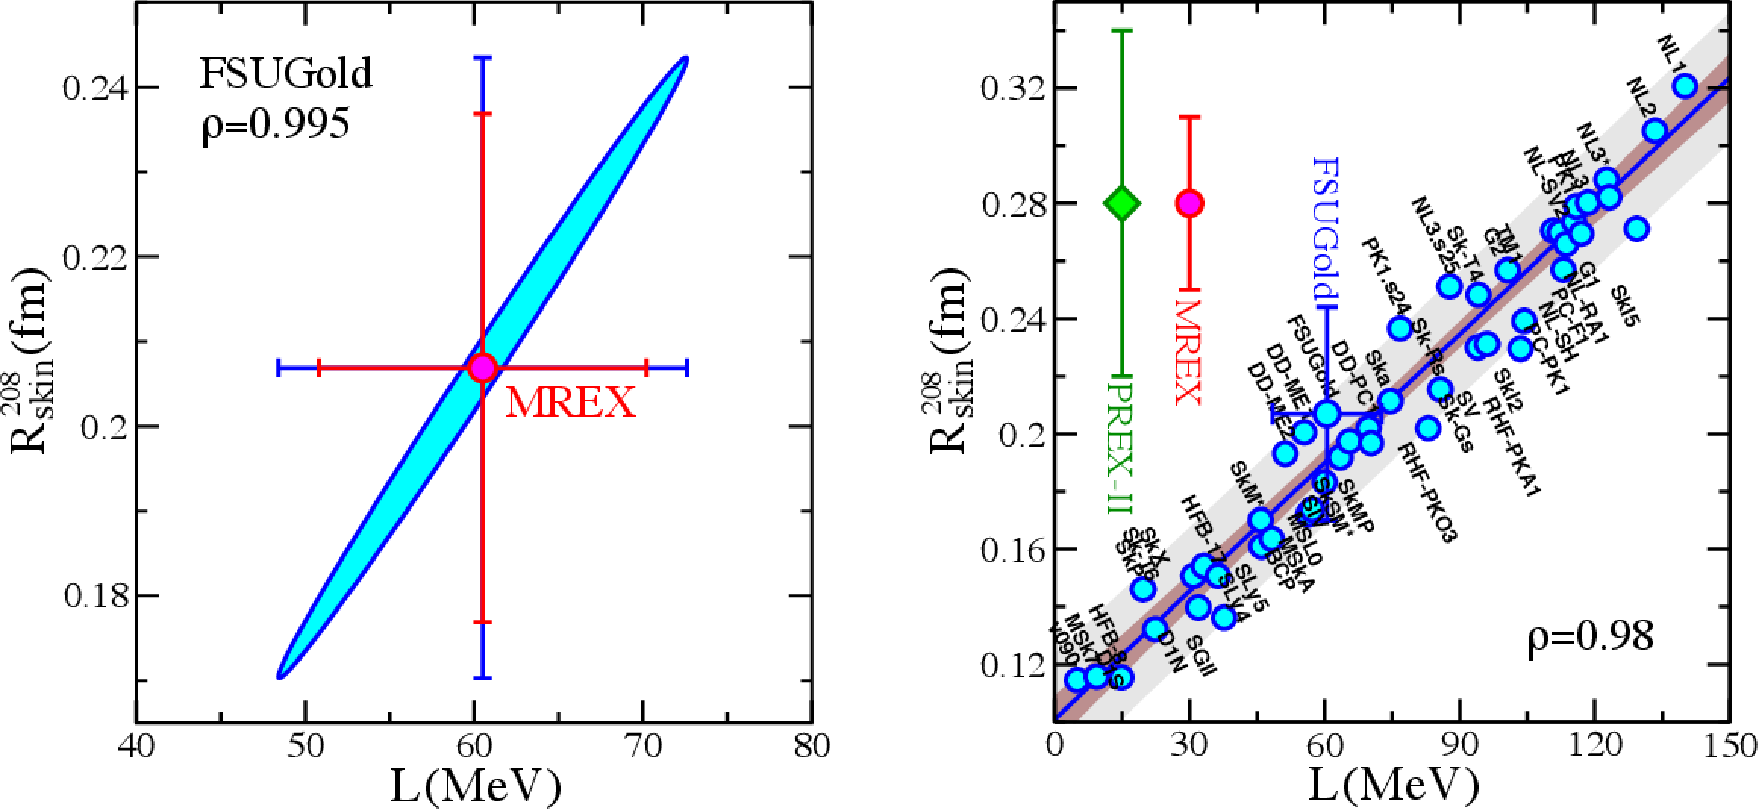
\includegraphics[width=0.75\textwidth]{Introduzione/LvsR.pdf}
 \caption{\textit{On the right} Neutron skin thickness of $^{208}Pb$ as a function of the slope of the symmetry energy $L$. Each dot represent the a value of $L$ and $\delta r_{np}$ as predicted by various theoretical models. The error bars represent $\pm \SI{0.06}{\femto \meter}$ and $\pm \SI{0.03}{\femto \meter}$ for the future experiments of PREX-II and MREX. Notice the different scale for x and y axis, a small uncertainty for the neutron skin measurement correspond to an higher uncertainty for the values of $L$. \textit{On the left} Covariance ellipse displaying the correlation between $L$ and the neutron skin thickness, for FSUGold model. The covariance $\rho$ is equal to 0.995.}
\label{fig:LvsR}
\end{figure}
 
A strong linear correlation is evident, then measuring the neutron skin gives access to $L$. 
  
\section{Parity-violating Scattering Experiment}

In the last years, the parity violating electron scattering seems to be a promising method for the determination of the neutron-skin thickness of $^{208}Pb$. The choice of lead is due to the significant neutron excess and stability of lead nuclei ($^{208}Pb$ is a double magic nucleus). The advantage of this method is that it is free from the many uncertainties associated to strong interaction. The main disadvantage is the need to accumulate large statistics, because the reaction are mediated by the weak interaction, associated with smaller scattering amplitude compared to electromagnetic and strong interactions. 
The parity violating scattering is highly sensitive to the neutron density because, as mentioned above, since the weak charge of the neutron is higher compared to the weak charge of the proton.
In this reaction, longitudinally polarized electrons are elastically scattered off a lead target. The important quantity to determine is the parity violating asymmetry $A_{pv}$, the difference in cross section between the scattering of right and left handed electrons. 

\begin{equation}
A_{pv} = \dfrac{\sigma_{R} - \sigma_{L}}{\sigma_{R} + \sigma_{L}} ,
\end{equation} 

The theoretical calculation of $A_{pv}$ includes the interference between the exchange of virtual $\gamma$ and $Z^{0}$. In the Born approximation $A_{pv}$ is directly proportional to the weak form factor, and is given by:

\begin{equation} \label{eq:BornLimit}
A_{PV} \simeq \dfrac{G_{F} Q^{2}}{4 \pi \alpha} \cdot \dfrac{Q_{W} F_{W}(Q^{2})}{Z F_{ch}(Q^{2})} ,
\end{equation} 

where $G_{F}$ is the Fermi constant, $Q^{2}$ is the transferred momentum, Z and $Q_{W}$ are the electric and weak charge of the nucleus, $F_{ch}$ and $F_{W}$ are the charged and weak form factors of the nucleus. The charge form factor of the lead nucleus is known with high accuracy (precision of 0.02 \%), so in this limit the only quantity that is unknown is $F_{W}(Q^{2})$. In the long wavelength approximation, the weak form factor at single value of momentum transfer is given by:

\begin{equation}
F_{W}(Q^{2}) = \frac{1}{Q_{W}} \int \rho_{W}(r) \dfrac{sin(Qr)}{Qr} d^{3}r = (1 - \frac{Q^{2}}{6} R^{2}_{W} + \frac{Q^{4}}{120}R^{4}_{W} + ...)  
\end{equation}

The form factor is normalized in such a way that $F_{W}(Q^{2} = 0) = 1$. The weak charge radius correspond to $R^{2}_{W} = -6 \frac{\partial F_{W}}{\partial Q^{2}}\Bigr|_{\substack{Q^{2} = 0}}$. Now it is clear that parity-violating experiment are a promising method to extract information about neutron density. The difficulty is represented by the small values of $A_{pv}$ asymmetry. Typical values are on the order of $1 \, ppm$ or less, for lead target. This requires high statistic to reduce the uncertainty of the measurement and high control over the systematic effects. In 2012 the PREX collaboration measured for the first time the neutron skin through parity-violating experiment, obtaining:

\begin{equation} \label{eq:Prex}
\delta r_{np} = 0.33^{+0.16}_{-0.18} \SI{}{\femto \meter}
\end{equation}

The error associated to this first measurement is not enough small to provide significant constraints on the values of $L$. The MREX experiment has the objective of measuring the neutron skin of lead with a precision of $0.5 \%$  ($\pm \SI{0.03}{\femto \meter}$). This high precision is needed to decrease the uncertainty associated to L. For example, the left plot in \ref{fig:LvsR}, shows the correlation between the neutron skin thickness of $^{208}Pb$ and the slope of the symmetry energy as predicted by FSUGold model (\cite{Fattoyev_2011}). With a precision of $\pm \SI{0.03}{\femto \meter}$, $L$ is determined with $\pm \SI{12.1}{\mega \electronvolt}$. 
In 2019, a new measurement of the PREX collaboration \cite{PREX:2021umo}, obtain of $\delta r_{np} = 0.283 \pm 0.071 \SI{}{\femto \meter}$. With the new measurement that will be performed in MESA accelerator by MREX, the precision will be improved further by a factor 2.

\subsection{Neutron Star Radius}

We mentioned that the slope of the symmetry energy $L$ is strongly correlated to the neutron skin thickness of $^{208}Pb$ and also to $R_{ns}$. We can go deeper in the discussion stating that the maximum neutron-star mass and radius are uniquely constrained by the E0S (\cite{Lindblom1992DeterminingTN}). The maximum mass depends on the energy density dependence of the pressure, that must be high enough to oppose the gravitational collapse into a black hole. Moreover, stellar radii are strongly dominated by the pressure of degenerate nuclear matter near the saturation density.  
The connection between the radius of compact object and pressure is enclosed in the Volkov-Oppenheimer equation (TOV) \cite{PhysRev.55.374} and in the equation of state; assuming a particular equation of state, it is possible to resolve the Volkov-Oppenheimer equation, finding the relation between neutron star mass and radius, or radius and pressure (formal proof in \cite{LATTIMER_2007}). 
The solution of the TOV equation for the simple case of a symmetric compact object, assuming a constant pressure over the entire volume of the neutron star, gives the relation between radius and pressure $P_{c}$ at the center of the star \footnote{This model is very simple and fails to describe the physics of a neutron star with accuracy, however it can be used to highlight the connection between pressure at the center of the star and radius}.

\begin{equation}
R^{2} = \dfrac{3}{8\pi \rho} \dfrac{1 - (\rho + P_{c})^{2}}{(\rho + 3 P_{c})^{2}}
\end{equation}

The pressure $P_{c}$ is, in large part, determined by the symmetry energy of the equation of state, so there should be a strong correlation between $L$ and the neutron star radius $R_{ns}$. In the end, different theoretical models \cite{PhysRevLett.95.122501} confirm the connection between $L$ and $R_{ns}$, for example we show the covariance ellipses predicted by FSUGold model between the slope of the symmetry energy $L$ and the stellar radii in figure \ref{fig:LvsRns}

\begin{figure}[hbtp]
\centering
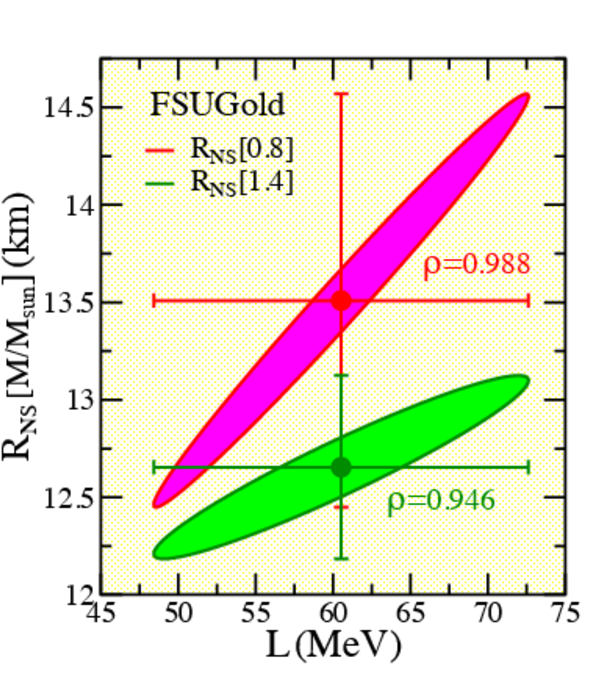
\includegraphics[width = 0.5\textwidth]{Introduzione/LvsRns.pdf}
\caption{Covariance ellipses between slope of the symmetry energy and stellar radii, for $0.8$ and $1.4$ solar masses, predicted by the relativistic density model FSUGold.}
\label{fig:LvsRns}
\end{figure}

From these consideration, astronomical observations of mass and radii of neutron stars represents important constrains on the EOS, and are valuable for understanding the behaviour and physics of the atomic nuclei.
Astronomical observations of the neutron star radius rely traditionally on photometric measurements, assuming that thermal emission of light from the surface follow a blackbody spectrum at uniform temperature. These measurement are affected by systematic uncertainties that are typically of a couple of kilometers.
However, the situation is rapidly changing with the beginning of the gravitational wave detection. The first observation of the binary neutron star merger by the LIGO-Virgo collaboration opened a new path to measure the neutron-stars radius \cite{LIGOScientific:2017vwq}. In fact, the gravitational wave generated by the merging of two neutron stars depends on a property called tidal deformability; this parameters describes the tendency of a neutron star to deform in response of the gravitational field of its companion star, developing a mass quadrupole moment. This parameters $\Lambda$, is highly sensitive to the ratio of the stellar radius to the Schwarzschild radius:

\begin{equation}
\Lambda = \frac{2}{3} k_{2} \big( \dfrac{c^{2} R_{NS}}{GM} \big)^{5}
\end{equation}

In this expression, M and $R_{NS}$ are the neutron star mass and radius, and $k_{2}$ is the second tidal Love number \cite{Binnington:2009bb}, which is computed from the quadrupole component of the gravitational field induced by the companion. From the first detection, an upper limit of $R_{NS}^{1.4} < \SI{13.76}{\kilo \meter}$ \cite{Fattoyev_2018} was placed on the radius of a neutron star with a $1.4$ solar masses. Because of the strong correlation between $R_{NS}$, $L$ and $\delta r_{np}$, this is a indirect constrain on the neutron skin thickness of $^{208}Pb$. An upper limit of $\delta r_{np} < \SI{0.25}{\femto \meter}$ was obtained. This limits is in slightly tension with the larger values measured by PREX collaboration, suggesting that the symmetry energy, for slightly higher density as in neutron stars, decreases with respect to the typical density found in atomic nuclei. This increment and decrement may be an indication of the presence of phase transition in the interior of neutron stars.

\begin{figure}[hbtp]
\centering
\includegraphics[width = 0.5\textwidth]{Introduzione/PolarizzabilitàR.png}
\caption{ Polarizability $\Lambda$ versus neutron star radius. The point are the prediction of different theoretical models. The upper bound with $90 \%$ credibility is shown in the figure. On the x axis, two variables are shown, the predicted neutron star radius and neutron skin thickness of lead.}
\end{figure}


\section{Transverse Asymmetry}

The parity-violating scattering has numerous advantages for extracting the neutron-skin thickness of nuclei. However, the asymmetry to measure is rather small. To measure such asymmetries, it is necessary to reduce as much as possible the systematic effects, that can alter the result of the measurement. One of the main sources of background for the measurement of $A_{PV}$ is a different process that concerns transverse polarized electrons. The different polarization of the electrons produce an asymmetry, called beam normal single spin asymmetry (BNSSA), or transverse asymmetry $A_{n}$. Since such asymmetries are typically one order of magnitude higher than the parity-violating ones, a small normal component of the beam polarization during parity-violating experiments can produce a systematic effect that changes the final result. The subject of this thesis is the measurement of transverse asymmetry $A_{n}$ for carbon target, performed at MAMI, the Mainz microton accelerator. The choice of carbon target is due to the fact that the transverse asymmetry for $^{12}C$ is well known and already measured at MAMI; the expected asymmetry is roughly $20 \, ppm$, thus it is particularly suited for the commissioning of the new experimental setup. Such asymmetries are challenging because they require calculation of box diagrams with intermediate excited states \cite{Gorchtein_2008}, which will be threated in chapter \ref{transv}. After the determination on $A_{n}$ for $^{12}C$, the next phase of the MREX experiment will be the determination of the transverse asymmetry for $^{208}Pb$. As already mentioned, this is mandatory to constrain the systematic effects in PV experiments. However, it is also interesting because in the last measurement performed by PREX \cite{HAPPEX:2012fud} the transverse asymmetry for $^{208}Pb$ target is compatible with zero, with a complete disagreement with the theoretical predictions. Since the theoretical prediction for hydrogen, helium, carbon and zirconium are in agreement with theory, a second, independent measurement of the BNSSA for lead is interesting, to confirm the measurement performed by PREX.  
